\documentclass{seal_thesis}

\usepackage{amsmath}
\usepackage[
  top=1.25in,
  bottom=1.25in,
  left=1.25in,
  right=1.25in
]{geometry}
\usepackage{tabularx,colortbl}

\thesisType{Master Project Report}
\date{\today}
\title{The Global Living Application Platform (GLAPP)}
\subtitle{}
\author{
Fabio Isler \textmd{(09-115-965)} \\
Man Wai Li \textmd{(14-705-156)} \\
Dinesh Pothineni \textmd{(14-707-988)} \\
Riccardo Patane \textmd{(09-177-270)}}
\home{} % Geburtsort
\country{}
\prof{Prof. Dr. Harald C. Gall}
\assistent{Dr. Philipp Leitner}
\email{}

\begin{document}
\maketitle

\abstract
Abstract


%%%%%%%%%%%%%%%%%%%%%%%%%%%%%%%%%%%%%%%%%%%%%%%%%%%%%%%%%
% NEW CHAPTER																						%
% Remember to always use a new line for a new sentence! %
%%%%%%%%%%%%%%%%%%%%%%%%%%%%%%%%%%%%%%%%%%%%%%%%%%%%%%%%%
\chapter{Introduction}\label{ch:introduction}

Cloud computing has created a paradigm shift in the last few years, by making infrastructure available at lower costs and with higher efficiency of operations.
These solutions are increasingly being adopted by enterprises and developers, as they can provision huge amount of resources to scale on-demand in order to meet their business needs.
In cloud computing, resources such as CPU processing time, disk space, or networking capabilities, are rented and released as a service.
Today, the most important model for delivering on the cloud promise is the Infrastructure-as-a-Service (IaaS) paradigm.
In IaaS, virtual computing resources are acquired and released on demand, either via an Application Programming Interface (API) or web interface.
Along with great flexibility of being able to get new resources on demand and pay for what you use, new problems arise.
Selecting a cloud service provider can often be a quite challenging decision for the developer or a company, so is being able to monitor and evaluate these infrastructure resources on a regular basis.
With so much of variance in cost and performance, it is imperative that one would look for a reliable deployment, monitoring solutions to strike a balance with application requirements.
Furthermore, the complexity and skill required to manage multiple layers of application, data, middleware and operating systems can be very high.

Understanding run time performance and behavior of various application components in realtime can enable us to take advantage of arbitrage opportunities that exist between different machines/regions or even other cloud providers.
For example, an application can take advantage by moving closer to its users based on timezones or traffic to improve response time.
Currently there is no flexibility to move freely between various cloud providers without great development effort and cost, however such an ability to move freely between providers enables us to benefit from cost and performance differences of cloud providers.
We propose a cloud middleware that can not only take care of application deployment to the cloud, but also constantly monitor and trigger necessary adaptations to benefit from these opportunities.
This middleware also enables developers to specify their intended goals in terms of high level policies to govern the application behavior.
The middleware can then break down these policies into low level objectives, in order to trigger adaptations by changing the state of application when required.

%%%%%%%%%%%%%%%%%%%%%%%%%%%%%%%%%%%%%%%%%%%%%%%%%%%%%%%%%
% NEW SECTION																						%
%%%%%%%%%%%%%%%%%%%%%%%%%%%%%%%%%%%%%%%%%%%%%%%%%%%%%%%%%
\section{Global Living Cloud Applications}

The aim of this project is to develop a platform for what we call \textit{global living cloud applications} (GLAs).
In a nutshell, GLAs are a bio-inspired notion of cloud-native applications.
GLAs live in the cloud, and are able to migrate between data centers and cloud providers automatically, based on changes in cost and performance of cloud offerings, changes in customer behavior or requirements, or other factors.

The bio-inspired terminology applies for the different levels of components of a GLA:

\begin{itemize}
	\item \textbf{GLA}: The GLA itself is a collection of organs that form the whole application.
	\item \textbf{Organ}: An organ consists of one or more cells and is responsible for a service.
	\item \textbf{Cell}: A cell is the lowest-level component of a GLA.
	There are two kinds of cells: The ones that provide user-defined functionality of the organ, and platform-defined cells like reverse-proxies for exposed ports
\end{itemize}


%%%%%%%%%%%%%%%%%%%%%%%%%%%%%%%%%%%%%%%%%%%%%%%%%%%%%%%%%
% NEW SECTION																						%
%%%%%%%%%%%%%%%%%%%%%%%%%%%%%%%%%%%%%%%%%%%%%%%%%%%%%%%%%
\section{GLAPP}

In order to manage these GLAs, we introduce a platform called GLAPP (\textbf{G}lobal \textbf{L}iving \textbf{AP}plication \textbf{P}latform).
It allows a developer to deploy multiple GLAs on whatever cloud she has access to and sets a centralized mechanism in place to constantly monitor and manage all the GLAs.
The platform supports heterogeneous environments, so a a GLA can live and move across different providers, regions, instance types, etc.

GLAPP is an open-source platform which can be deployed easily on a server. Set-up instructions can be found on github\footnote{https://github.com/glapp/gla-sails}, as well as all the source code that was developed in the course of this project\footnote{https://github.com/glapp}

%%%%%%%%%%%%%%%%%%%%%%%%%%%%%%%%%%%%%%%%%%%%%%%%%%%%%%%%%
% NEW SECTION																						%
%%%%%%%%%%%%%%%%%%%%%%%%%%%%%%%%%%%%%%%%%%%%%%%%%%%%%%%%%
\section{Outline}
This report serves the purpose of giving an overview of the whole project.
In chapter~\ref{ch:background}, we give some background information about design and implementation decision as well as the architecture of GLAPP.
Chapter~\ref{ch:components} introduces all the components GLAPP consists of in more detail.
In chapter~\ref{ch:casestudy}, we present the case study we had in mind and demoed in our final presentation.
Chapter~\ref{ch:futurework} discusses possible extensions and future work on the project.
The report is concluded in chapter~\ref{ch:conclusion}.



%%%%%%%%%%%%%%%%%%%%%%%%%%%%%%%%%%%%%%%%%%%%%%%%%%%%%%%%%
% NEW CHAPTER																						%
% Remember to always use a new line for a new sentence! %
%%%%%%%%%%%%%%%%%%%%%%%%%%%%%%%%%%%%%%%%%%%%%%%%%%%%%%%%%
\chapter{6 PAGES: Background \& Architecture}\label{ch:background}

%%%%%%%%%%%%%%%%%%%%%%%%%%%%%%%%%%%%%%%%%%%%%%%%%%%%%%%%%
% NEW SECTION																						%
%%%%%%%%%%%%%%%%%%%%%%%%%%%%%%%%%%%%%%%%%%%%%%%%%%%%%%%%%
\section{Basic Design Decisions}
\todo{IN CHARGE: Adrian}

\subsection{Main Components: Provisioning Backend, Frontend, Control Loop}
GLAPP consists of three building blocks: A provisioning backend, a frontend and a control loop.
In developing GLAPP, we made different decisions in platform architecture as well as implementation.
Docker containerization is the infrastructure backbone where the GLAs are deployed to.
GLA deployment on this infrastructure is handled by the provisioning backend.
It is implemented with node.js runtime and Sails framework.
The second component is the frontend.
It provides an interface for the user to interact with the platform.
While is also developed with node.js runtime, AngularJS framework is used.
Lastly, a control loop following the Monitoring, Analysis, Planning and Execution (MAPE) model is developed using Java with BURLAP library and framework.

\subsection{Deployment: Containerization with Docker}
\subsubsection{Containerization vs. other virtualization methods:}
We set out to create a platform to manage GLAs.
Speed of deployment is therefore an important criterion when considering the underlying technology.
While both virtual machine and containerization are virtualization technologies that provision shared cloud computing resources, virtual machine focus on virtualization of infrastructure resources and containerization focus on virtualization of platform \todo{add reference}.
Being a lightweight virtualization technology, containerization gets rid of the guest OS layer as in traditional virtual machine architecture.
Instead, applications are deployed on top of a container engine which runs on host OS.
In addition, application binaries are stored in a package along with the necessary libraries in the case of containerization.
This contrasts to the full OS required for a virtual machine.
These lightweight runtime and packaging provides a fast deployment that is a crucial aspect of GLAPP.
With this containerization techology, GLAPP can deploy application components in seconds when the application images are present on the host.
In addition to the fast deployment, containerization has a much smaller footprint comparing with virtual machines.
A normal virtual machine image has a size in gigabytes due to the presence of a full OS.
In contrasts, a container image used in our case study take up only a few hundred megabytes as it only includes the application binaries and required libraries.

% full os vs packaged binary and library

%\todo{Explain the advantage of containerization compared to e.g. virtual machines}
%@Adrian: Some resources that help understand this difference
%\begin{itemize}
%	\item http://searchservervirtualization.techtarget.com/answer/How-is-containerization-different-from-virtualization
%	\item https://jaxenter.com/containerization-vs-virtualization-docker-introduction-120562.html
%\end{itemize}

%In general, i think the following points can be stated here:
%\begin{itemize}
%	\item Containerization is much more lightweight. Some MB for a container compared to some GB for a whole VM
%	\item This enables faster deployment, which is crucial to our problem
%	\item Disadvantage of containerization is that the containers are less isolated than a whole VM. However, for a student project, such security questions are less important and new developments in current containerization implementations like Docker seem to handle isolation quite well.
%\end{itemize}


\subsubsection{Docker vs. other containerization technologies:}
In containerization, there are various models and technologies.
For example, both Docker and OpenVZ are containerization technologies but they use different models.
However, Docker container functions as an application or a service while OpenVZ container functions as a virtual private server (VPS) for deploying additional application stack on top of it \todo{add reference https://openvz.org/Main\_Page}.
Similar to OpenVZ, LXD is another machine containerization technology \todo{add reference}.
As GLAPP aims at managing GLAs, Docker provides the most direct way of containerization of application.
With other containerization technologies like OpenVZ or LXD, the platform will need to manage both the application deployment on those containers as well as deployment of the container on cloud infrastructure.
This adds another layer of overhead and complexity.

%\todo{Explain the advantage of Docker compared to e.g. OpenVZ}
%\begin{itemize}
%	\item Basically, Docker was a big hype in the early stage of our project, and keeps being in the news until today -> nice to work on a bleeding-edge technology
%	\item There are many similarities between all these containerization implementations, but I think docker is the most straight-forward application containerization (for web-applications / services). E.g., LXD focuses more on the deployment of virtual machines as containers (yes, now it gets inception-like :P)
%	--> See http://unix.stackexchange.com/questions/254956/what-is-the-difference-between-docker-lxd-and-lxc
%\end{itemize}

\subsection{Orchestration: Docker Swarm}
%\todo{Explain the advantage of Docker Swarm compared to e.g. Kubernetes}
For GLAPP to manage the GLAs in response to the needs of application or changing environment, GLA need to be run in form of a cluster across different cloud computing resource.
Docker Swarm is the orchestration tool used to manage this cluster of containers.
Orchestration tool is used to control the deployment of containers across the cloud infrastructure to satisfy various objective such as load-balancing.
While there exists other tools such as Kubernetes that provides orchestration functionalities, Docker Swarm provides additional capability to manage hosts of different cloud service providers.
For example, Docker Swarm can also create and delete of hosts and mange the members of the cluster.
This enables extension possibility of MAPE to manage not only the containers, but also underlying cloud computing resources.

\subsection{Rule-Based Adaptations vs. Markov Decision Process}
\todo{To be reviewed by: Riccardo}
%\todo{Explain the thought process behind this decision}
Markov Decision Process (MDP) and rule-based adaptations are for determining appropriate adaptation action to change application from an undesired state where policy is violated to a desired state where the policy is fulfilled.
In reinforcement learning, a reinforcement learning problem is defined as the problem of learning from interaction to achieve a goal \todo{add reference}.
MDP is a reinforcement learning task that satisfy the Markov property \todo{add reference}.
During the development of GLAPP, Q-Learning was implemented as a method of MDP to determine the adaptation action.
However, due to the problem nature, there is a high number of state is resulted from large amount of features in modelling the GLAs.
This leads to an ineffective Q-Learning when lookup table is used for Q-values.
Details of this problem is discussed in Markov Decision Process section of Components chapter (section 3.3.4).
As a result, rule-based adaptations was used in the final implementation.
Instead of a reinforcement learning approach, heuristic is used for adaptation action determination.
Rule-based adaptation is fast in finding adaptation action to address violated policy comparing with Q-Learning when lookup table.
This is because adaptation action generated by rule-based adaptation will be effective when the rules are well-defined.
In contrasts, MDP requires the convergence of Q-values in order to generate effective adaptation actions.
At the same time, the heuristic rules used are easy to understand for further tweaking.
However, rule-based adaptation also has its disadvantages.
For instance, it does not scale well as the types of metric or the complexity of policy due to additional rules are required when new types of metric are introduced or the policy becomes more complex.
In such case, MDP will scale well as the Q-value will converge learnt over time.
That means even with additional metrics and complex policy, once Q-Learning have the converged Q-values, it is expected to generate effective adaptation action.

%%%%%%%%%%%%%%%%%%%%%%%%%%%%%%%%%%%%%%%%%%%%%%%%%%%%%%%%%
% NEW SECTION																						%
%%%%%%%%%%%%%%%%%%%%%%%%%%%%%%%%%%%%%%%%%%%%%%%%%%%%%%%%%
\section{Implementation Decisions}
\subsection{Backend: Node.js}
The backend has been implemented with the \textit{Node.js}\footnote{https://nodejs.org/} runtime.
More specifically, we used a framework called \textit{Sails}\footnote{http://sailsjs.org/}.
Although it is labeled as a complete MVC framework, we mainly used it to implement the server-side functionality and to provide a clean REST for the other GLAPP components.

There are two reasons why we chose Node.js and Sails in particular.
For one thing, it was the backend framework some of us were most experienced in, which made it easier to focus on the actual project without having to work our way into a new framework.
For another thing, Node.js comes with the well-established packaging system \textit{npm}\footnote{https://www.npmjs.com/}, where we found very helpful packages for our problem domain.
As an example, \textit{dockerode}\footnote{https://www.npmjs.com/package/dockerode} was the module which we used to implement the Docker-specific functionality, and it proved to be very well maintained, adding new functionalities whenever a new Docker release was published.
Since we were about to work with relatively new technologies like Docker, it seemed reasonable to count on packages which we knew will be adapted to changes in these new technologies.

\subsection{GUI: AngularJS}
\todo{DONE BY: Dinesh}
\todo{Explain the choice and alternatives}


This component of the application facilitates users to interact with rest of the platform. 
Since the whole back-end already provides REST endpoints for all the services, platform is fairly relaxed in choosing a framework for the front-end. 
Angular was particularly chosen for two important reasons. 
Since we had already decided to use node.js for the server component, it helps a great deal in terms of productivity to be able to use the same language for other components. 
Team could easily switch between the server and front-end while developing features. 
This can greatly aid us to iterate faster on the feedback received. 

Some of the benefits of using Angular framework are as follows. 
Data binding is the foremost advantage in the application, meaning any dynamic fields in the interface can be watched and automatically updated as the new data comes in. 
Directives for DOM manipulation and two way data binding makes a lot of known hardships a breeze with angular. 
Angular code can be very modular, reusable with easy to test features. 
Template system provides great reusability of various components. 
We used Bower and NPM for package management, as they provide comprehensive set of libraries for all the application needs. 
Routing is built-in to angular, which makes a single page application possible. 
This can make an application run extremely smooth and fast, once its loaded on the browser. 
Directives are very useful to define custom HTML tags and reuse the most frequent features in the views. 
In addition to this, modularity, abstraction of services makes a strong case for Angular. 
Last but not least, it is supported and maintained by Google, which can guarantee a long term road map and future development of the framework.

\subsection{MAPE: Java}
\todo{To be reviewed by: Riccardo}
\todo{Explain the choice and alternatives}
Java is a widely used programming language with good interoperability and decent support by other system or libraries used in this project.
MAPE is a key component of the GLAPP platform.
One of the important aspect of MAPE is the ability to easily interface with other components and system inside or outside GLAPP platform.
Another consideration is the availability of third party libraries that GLAPP can leverage to perform common computation using well-known algorithm such as various planning and learning algorithms used in Markov Decision Process (MDP).

A set of comprehensive functionality is provided through Java API and third party libraries.
In addition to functionality included in Java standard API such as HTTP connection used for interfacing with SAILS backend and monitoring system, useful third party libraries are also available.
For instance, GSON library \footnote{https://github.com/google/gson} provides easy API to create and manipulate JSON objects that is used for data exchange between MAPE and SAILS backend as well as between MAPE and monitoring system.
Most importantly, BURLAP library \footnote{http://burlap.cs.brown.edu/} provides not only a set of planning and learning algorithm for Markov Decision Process in reinforcement learning, but also a framework for further extending the processing capability through custom implementation of various components including learning algorithm and approximation function.
Availability of these functionalities from built-in and third party library makes Java a compelling language in developing MAPE component.


%%%%%%%%%%%%%%%%%%%%%%%%%%%%%%%%%%%%%%%%%%%%%%%%%%%%%%%%%
% NEW SECTION																						%
%%%%%%%%%%%%%%%%%%%%%%%%%%%%%%%%%%%%%%%%%%%%%%%%%%%%%%%%%
\section{Architecture}
The platform consists of 3 different parts/blocks: a frontend, a server backend and a control loop.
The frontend provides an interface for developer to interact with the middleware to deploy and manage her GLAs.
The server backend provides the management functionalities of the middleware including cloud infrastructure management, application deployment and access to the application status information.
Lastly the control loop is the component responsible for enabling the management of GLAs by the platform itself.
It follows the MAPE (Monitoring, Analysis, Planning and Execution) principle.
Possible execution actions are moving cells between different cloud instances (migration), duplicating/splitting cells of the GLA (mitosis), or removing cells.

\begin{figure}[!ht]
\centering
	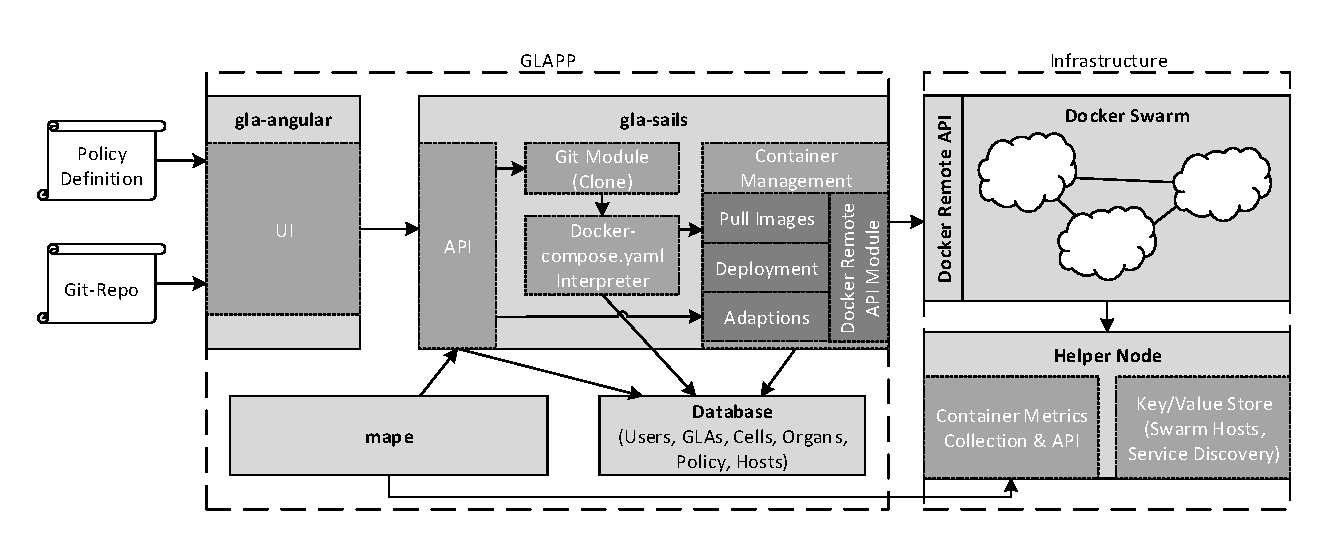
\includegraphics[width=\textwidth]{detailed_architecture.pdf}
	\caption{Detailed Architecture of GLAPP and the Infrastructure}
	\label{fig:detailed}
\end{figure}
\todo{Explain the separate parts - DONE BY: Dinesh}


Going into the details of architecture, GLAPP platform is designed to be modular and interoperable from the very beginning. 
Every component is connected to each other through a series of API calls, so that every critical component in the platform can be modified without large dependency chains, or even completely replaced with a better one if needed.
A simple user interaction flow through the platform architecture looks as follows. 
Once the developer decides to use the platform, they interact with the user interface (UI) to create a new global living application (GLA). 
One can create a new GLA by simply providing the URL address of their code repository. 
If it's a valid repository, front-end module passes the repository URL to the sails server through API. 
Git Module in the sails server then clones this repository to find the compose file. 
Platform presumes that this repository contains a docker compose file, which is a means of specifying configuration of main components in their application. 
The structure of this compose file specifies the important services in the application, the sources of each of their images, various environment variables, ports to be exposed and dependencies to make them run smoothly. 
Docker Interpreter module will perform this task of analyzing the compose file and storing the necessary information into the database. 
It creates the high level definition of the GLA, with its main organs and other important information.
	
Database module is responsible for storing every piece of information related to the application, users, except the cell images themselves. 
This is handled by the docker remote API, which is a part of container management module. Container management is an important liaison between the infrastructure and the sails server. 
It is responsible for pulling images mentioned in the compose file and storing them in the infrastructure, in a ready to deploy state. 
It also executes the initial deployment and any future changes to deployment in terms of adaptations. 
Each image pulled from the compose file is stored as an elementary cell, from which future cells of the GLA are created. 
Each cell stored in the infrastructure can be re-used if any other GLA's has a specification of the same cell. 
For example, if your GLA has a postgres database mentioned as a cell this will be stored and made readily available for any other GLA's using the postgress cell. 
In this way, we cut down the waiting time for images to be pulled down to a fraction of what it would usually take and many GLA's can be created and deployed instantaneously in the cloud.

Infrastructure is the bottom layer in GLAPP platform. 
Our architecture uses docker swarm technology underneath to create a cluster of servers across various cloud providers with a common internal network routing in place. 
This allows us to have servers in any part of the world, or with any provider like Google, Amazon, Digitalocean and still be able to talk to each other as they are part of one entity. 
In the cluster, there is one swarm master and multiple swarm-agents which talk to each other through the swarm master. 
We deployed a key value store in one of host machines to keep track of the host information. 
Consul application is used to help with service discovery and keep track of any changes. 
Registrator is used along with consul as a service registry bridging tool, to automatically register and deregister services of any cells as they become on-line or off-line. 
Whole infrastructure cluster with multiple hosts, and application services running inside these host machines are organized into one major module. 
This infrastructure module communicates with sails server through the remote API. 

Additionally we also use Prometheus, a powerful monitoring solution and a time series database to feed our application metrics data. 
In order to make this happen, we run a prometheus agent on every host machine, which periodically monitors all the containers that are currently running on a particular host to feed respective data into this time series database. 
We use cAdvisor for this function. 
It is a daemon, that collects information related to the resource usage, network statistics and performance of the running containers in the machine. 
It has native support for docker containers, which makes it a perfect bid for the job. 
Prometheus server scrapes data from all agents every few seconds. 
Best part is, prometheus not only collects the data, but also provides a powerful query language to aggregate and query the metric data. 
This monitoring module is also extensible with external application metrics, as REST API is built into the prometheus tool. 
GLAPP platform facilitates a way to feed third party application metrics into the platform, with the help of this.

During the creation of a new GLA, a developer can specify high level application policies to guide their GLA's. 
For example, a policy related to cost can be set as not to exceed 1USD/hr, irrespective of the load or the number of cells running at the moment. 
It's then the job of GLAPP platform to continuously optimize deployment strategy, so that this policy is never breached. 
Theoretically meaning, it should strike a balance between cheaper instances, high availability in all regions for the users while ensuring other goals if there are any. 
This is where MAPE comes into the picture. 
It serves as the nucleus of the platform. 
As soon as the application is deployed, MAPE looks for policies set on the GLA. 
If there are any, it then retrieves the related application metric data from the prometheus server. 
Analysis module then compares the policies with metric data to detect if there are any current violations. 
In the event of a violation, planning module then recomputes the optimal deployment strategy and necessary adaptations to achieve that goal. 
Execution module then executes the planned adaptations by communicating the specifics to the sails server, which then executes the actual changes in the infrastructure. 
Planning module is the crucial step here, and this is extensible. 
Meaning, one can swap this part with a different planning algorithm of their choice to optimize the deployment. 
Currently MAPE supports a basic form of markov decision process using Q-learning and a rule based algorithm. 
This whole cycle of monitoring, analysis, planning and execution is repeated until the application reaches a healthy state. 
It ensures the application is always healthy and adheres to the set policies. 
More details on the individual components and their implementation follows in the coming chapter.


%%%%%%%%%%%%%%%%%%%%%%%%%%%%%%%%%%%%%%%%%%%%%%%%%%%%%%%%%
% NEW CHAPTER																						%
% Remember to always use a new line for a new sentence! %
%%%%%%%%%%%%%%%%%%%%%%%%%%%%%%%%%%%%%%%%%%%%%%%%%%%%%%%%%
\chapter{10 PAGES: Components}\label{ch:components}

%%%%%%%%%%%%%%%%%%%%%%%%%%%%%%%%%%%%%%%%%%%%%%%%%%%%%%%%%
% NEW SECTION																						%
%%%%%%%%%%%%%%%%%%%%%%%%%%%%%%%%%%%%%%%%%%%%%%%%%%%%%%%%%
\section{Backend}

The backend is mainly responsible for the deployment and is the central component that defines the data structure of the platform. In order to understand the main functionality of the backend server, this section introduces the data models, the REST API, the services and the tests of this component.

\subsection{Data Models}
Figure~\ref{fig:models} provides a simple ER-like overview over the way how the server stores the data about users, applications, etc.
The mentioned attributes are exemplary, but represent the most important ones to understand the whole model.
It is apparent that the model is tightly coupled to the introduced notion of a GLA - an application which consists of organs, which again consist of cells.

\begin{figure}[!ht]
\centering
	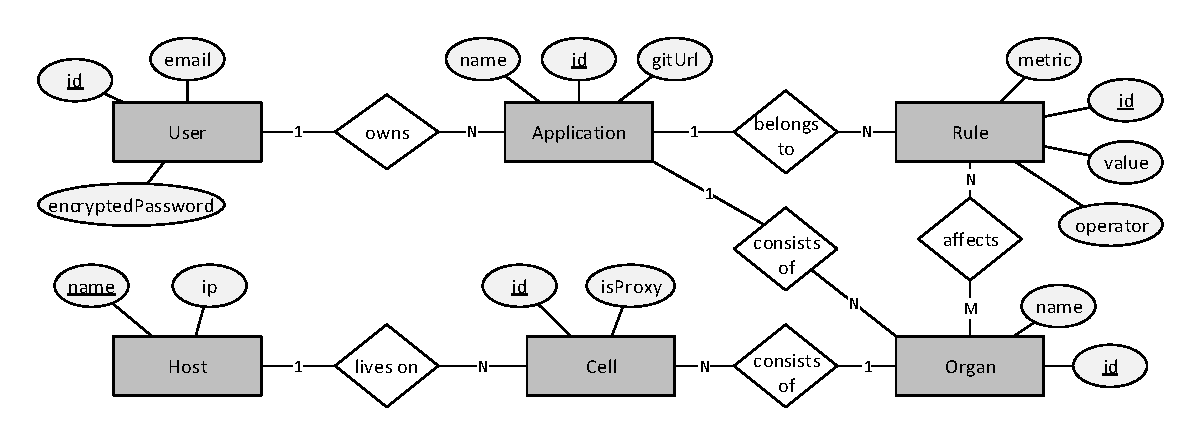
\includegraphics[width=\textwidth]{models-overview.pdf}
	\caption{Simple overview over the models and their relations}
	\label{fig:models}
\end{figure}

Sails is built upon an ORM called \textit{waterline}\footnote{https://github.com/balderdashy/waterline}, which allowed us to manage the data on a relatively high level.
That means that by defining the models and their relations and by setting up a connection to any database in the configuration of Sails, the data could be stored and retrieved by simple function calls.
We decided to use \textit{MongoDB}\footnote{https://www.mongodb.com/community} as a database.

\subsection{REST API}
The backend is supposed to serve the frontend and the MAPE component with data and to provide an interface for triggering adaptations to the deployment.
To achieve this clean interface, there is a REST API in place. Table~\ref{tab:endpoints} lists and describes the endpoints of this API.
Since our components are completely modularized and the communication only happens via this interface, the remaining components like the frontend or the MAPE are easily interchangeable.

\begin{table}
	\renewcommand{\arraystretch}{1.2}
	\caption{Endpoints of the REST API}\label{tab:endpoints}
	\begin{tabularx}{\textwidth}{|l|X|}
		\hline
		
		%%%%% Header
		\textbf{Endpoint}
			& \textbf{Description}
			\\ \hline
		
		%%%%% User
		\rowcolor[gray]{0.9}
		\multicolumn{2}{|c|}{User} 
			\\ \hline
		\textit{POST /user/signup}
			& Used by the frontend to sign up a user.
			\\ \hline
		\textit{PUT /user/login}
			& Used by the frontend to log in a user.
			\\ \hline
		\textit{GET /user/logout}
			& Used by the frontend to log out a user.
			\\ \hline
		\textit{GET /user/confirm-login}
			& Helper endpoint needed for the frontend to assure a user stays logged in on a refresh of the page.
			\\ \hline

		%%%%% Application
		\rowcolor[gray]{0.9}
		\multicolumn{2}{|c|}{Application} 
			\\ \hline
		\textit{GET /application/getUserApps}
			& Used by the frontend to get high-level information about applications of a specific user.
			\\ \hline
		\textit{GET /application/details}
			& Used by the frontend to get detailed information of a specific application.
			\\ \hline
		\textit{POST /application/add}
			& Used by the frontend to add an application.
			\\ \hline
		\textit{POST /application/remove}
			& Used by the frontend to remove an application, including clearing up its existing cells on the hosts.
			\\ \hline
		\textit{POST /application/deploy}
			& Endpoint used by the frontend to deploy an application on the infrastructure.
			\\ \hline
		\textit{POST /application/undeploy}
			& Used by the frontend to clear up an application's existing cells on the hosts.
			\\ \hline
		\textit{POST /application/rename}
			& Used by the frontend to rename an application.
			\\ \hline
		
		%%%%% Organ
		\rowcolor[gray]{0.9}
		\multicolumn{2}{|c|}{Organ} 
			\\ \hline
		\textit{POST /organ/scaleUp}
			& Used by the MAPE to scale up an organ. Constraints can be defined to place the new cell on a specific host, e.g. in the region ``US``.
			\\ \hline
		\textit{POST /organ/scaleDown}
			& Used by the MAPE to scale down an organ. A specific cell can be specified to control what cell is going to be destroyed.
			\\ \hline
			
		%%%%% Cell
		\rowcolor[gray]{0.9}
		\multicolumn{2}{|c|}{Cell} 
			\\ \hline
		\textit{POST /cell/move}
			& Used by the MAPE to move a specific cell from one host to another.
			\\ \hline

		%%%%% Host
		\rowcolor[gray]{0.9}
		\multicolumn{2}{|c|}{Host} 
			\\ \hline
		\textit{GET /host/info}
			& Used by the MAPE and the frontend get information about the current infrastructure.
			\\ \hline
		\textit{GET /host/prometheusUrl}
			& Used by the MAPE get obtain the URL of Prometheus.
			\\ \hline
			
		%%%%% Rule
		\rowcolor[gray]{0.9}
		\multicolumn{2}{|c|}{Rule} 
			\\ \hline
		\textit{GET /policy}
			& Used by the MAPE and the frontend to get the list of rules for a specific application.
			\\ \hline
		\textit{POST /policy/set}
			& Used by the frontend to set a new or replace an existing rule.
			\\ \hline
		\textit{POST /policy/remove}
			& Used by the frontend to remove a rule.
			\\ \hline
		
		%%%%% Analytics
		\rowcolor[gray]{0.9}
		\multicolumn{2}{|c|}{Analytics}
			\\ \hline
		\textit{GET /analytics/organCpu}
			& Used by the frontend to retrieve organ-level data for the cpu usage graph.
			\\ \hline
		\textit{GET /analytics/organMemory}
			& Used by the frontend to retrieve organ-level data for the memory usage graph.
			\\ \hline
		\textit{GET /analytics/events}
			& Used by the frontend to retrieve application-level data for the events graph.
			\\ \hline
	\end{tabularx}
\end{table}

\subsection{Services}
In the Sails framework, services are used to handle specific, API-independent functionalities.
For most of the internal logic apart from the actual API of the backend server, we created the following two well-encapsulated services:
\begin{itemize}
	\item \textbf{DockerService}: \\
	The DockerService is responsible for all the low-level, docker-specific functionalities.
	Many of the requests mentioned in table~\ref{tab:endpoints} trigger quite complex actions.
	For example, when a user requests to deploy an application, the server generally handles the following steps:
	(1) Creating an overlay network on the hosts,
	(2) Creating all the necessary cells in this network, and
	(3) Creating a reverse proxy cell for each organ that has an exposed port.

	To avoid such low-level logic in the API controllers, it makes sense to encapsulate this in a service.
	The DockerService handles the connection to the Docker infrastructure by the mentioned npm package \textit{dockerode}.
	It takes care of everything that is concerned with Docker, consisting of the following categories:
	\begin{itemize}
		\item Initialization: Establishing the Docker infrastructure connection, extracting the organs from the initial docker-compose.yml file
		\item Deployment: Handle the overlay network, deployment (creating the containers and the reverse proxies as cells)
		\item Adaptations: Moving containers, adding/removing containers, clearing all containers of a certain application
		\item Infrastructure: Get host information and parse it in order to save it in our database
	\end{itemize}
	
	\item \textbf{PrometheusService}: \\
	The PrometheusService is responsible for a clean provisioning of analytic data for the frontend.
	It establishes the connection to the Prometheus API and allows the fetching of any data the user requests.
	Since this data is cell-level data, it makes sense to have aggregation functions in place.
	In the current version of this service, only \textit{average} is implemented, but it's programmed in a pipeline-like way so various alterations and aggregations of the data can be added and chained to the service call.
\end{itemize}


\subsection{Tests}
It is crucial for the whole platform that the backend's interface works as expected.
To assure this, we wrote tests of all the API endpoints in different scenarios, based on the Node.js testing framework Mocha\footnote{https://mochajs.org/}.
Since most requests trigger functions of the services, these tests cover the majority of code in the backend.
How to run the tests is described in the README.md\footnote{https://github.com/glapp/gla-sails} of the backend component.


%%%%%%%%%%%%%%%%%%%%%%%%%%%%%%%%%%%%%%%%%%%%%%%%%%%%%%%%%
% NEW SECTION																						%
%%%%%%%%%%%%%%%%%%%%%%%%%%%%%%%%%%%%%%%%%%%%%%%%%%%%%%%%%
\section{2 PAGES: GUI}
\todo{DONE BY: Dinesh}


%%%%%%%%%%%%%%%%%%%%%%%%%%%%%%%%%%%%%%%%%%%%%%%%%%%%%%%%%
% NEW SECTION																						%
%%%%%%%%%%%%%%%%%%%%%%%%%%%%%%%%%%%%%%%%%%%%%%%%%%%%%%%%%
\section{MAPE}
\todo{To be reviewed by: Riccardo}
MAPE is the control loop of the platform and responsible for managing the deployed applications in accordance to the policy.

% add a detailed description of the problem?

It analyzes the environment information and performance metrics to determine the healthiness of application and trigger appropriate adaptation action should there be any violation to the policy.
The environment information includes details of the infrastructure, application deployment and user-defined policy.

MAPE consists of three parts: one interfaces with other systems to retrieve the necessary information for analysis and dispatch the adaptation action, another part analyzes the application status and determine its healthiness with regard to the policy, and the last part determines appropriate adaptation action based on the environment information and the computed healthiness.

MAPE implementation are grouped into several packages:
\begin{itemize}
\item Package \texttt{ch.uzh.glapp} contains the core classes of MAPE including \texttt{MainLoop} class where the main function is defined.
It also include classes for interfacing with other systems as well as an utility class providing auxiliary functions used in various computation. 
\item Package \texttt{ch.uzh.glapp.mdp} contains the classes for MDP using BURLAP library.
\item Package \texttt{ch.uzh.glapp.model} and its subpackages contain the classes for modelling the infrastructure information and performance metrics returned by SAILS backend and monitoring system.
\end{itemize}

\subsection{Interface with other systems}
At the start of each control loop, MAPE interfaces with SAILS backend to retrieve environment information, and with monitoring system to retrieve performance metrics. On the other hand, MAPE communicates to SAILS backend to execute the adaptation action.
As mentioned in the implementation decision section, MAPE use HTTP protocol with JSON object for data exchange.
It retrieves the infrastructure, application deployment information and user-defined policy from SAILS backend as well as performance metrics through HTTP requests.
For instance, infrastructure information includes information of virtual machines such as the service provider, machine location and machine tier. Deployment information, on the other hand, refers to the information of each application components including on which containers they are currently deployed.
Furthermore, MAPE also retrieves user-defined policy through SAILS backend. A policy is set of rules that defines which metrics the application need to comply to, its threshold for healthiness determine and the weight of each rule relative to the others.
Lastly, MAPE retrieve the performance metrics from the backend monitoring system.
JSON objects are used for all these information retrieval.
The use of JSON objects provides a data structure that is flexible to represent different types of information from different interfacing systems.
In addition, it allows MAPE to build a object-oriented view of the whole environment that provides quick access to specific information for various computations.

\subsection{Policy}
Policy is a key element for MAPE.
It consists of a set of user-defined rules that governs the application deployment.
A rule is specified with the following information:
\begin{itemize}
\item \textbf{metric} defines performance indicator that the current deployment will be measured against.
\item \textbf{organ} defines the organ(s) that the rule is applicable to.
\item \textbf{threshold} defines the upper or lower bound that the metric value should be compliant to.
\item \textbf{operator} defines how the metric value should be compared to the threshold.
For example, a "less than" operator means the metric value need to be less than the specified threshold.
\item \textbf{weight} defines the weight of a rule relative to others when multiple rules are specified.
\end{itemize}
Based on the metric selected, a rule can be classified into one of the following three types:
\begin{itemize}
\item \textbf{Resource utilization rule} limits the resource utilization to the specified threshold.
An example would be to restrict the CPU utilization to be lower than 80\%.
\item \textbf{Cost rule} limits the total cost incurred from running on the cloud infrastrcture.
\item \textbf{Application metric rule} specifies the range of application metric that the application need to comply to.
In current implementation, click rule is an example of application metric rule.
\end{itemize}

\subsection{Healthiness Computation}
Based on the rules defined in the policy, healthiness is computed.
For the $i$-th rule, the healthiness of a cell is defined as the ratio of the difference between metric value and threshold to the threshold normalized with the weight of the rule:
\[ \textrm{healthiness}_{cell} = \frac{\textrm{difference between metric value and threshold}}{\textrm{threshold}} \times \frac{w_i}{\sum_{i=1}^{n}{w_i}}\]
where $w_i$ is the weight of the $i$-th rule and $n$ is the total number of rules.

A positive healthiness value means the metric value is compliant and a negative healthiness value means the metric value is non-compliant.
For example, assume there is only one rule, if the rule specifies the "CPU utilization" need to be "less than" a threshold of 0.8 (80\%) and the current CPU utilization is 0.6(60\%), the healthiness value will be:
\begin{align*}
\textrm{healthiness} &= \frac{0.8 - 0.6}{0.8} \times \frac{1}{1}\\
&= 0.25
\end{align*}
%The healthiness value of a rule is the aggregated value of all cells' healthiness values:
%\[ \textrm{healthiness}_{rule} = \sum_{i=1}^{n}{h_i}\]
%where $h_i$ is the healthiness value of the $i$-th cell and $n$ is the total number of cells applicable under a given rule.
The healthiness value of a rule is the aggregated value of all cells' healthiness values.

After the healthiness values of the each individual cell is computed based on the policy and performance metric, all violating cells within an organ are taken into account for an evaluation.
When the number of violating cell exceed a defined threshold, the rule will be considered as violated.
Information of each violating cell along with the healthiness value will added to a list of violations.
This list of violations will be further processed in MAPE to determine appropriate adaption action.

% add details about the processing the violation information

\subsection{Markov Decision Model}
% burlap library for MDP and its extensibility
Markov Decision Model (MDP) will be triggered to find an application deployment that fulfil policy requirement whenever a rule violation is detected.
In the first implementation of MAPE, MDP as a reinforcement learning process was used to solve the problem of determining adaptation action in response to the rule violation.
The output of solving this problem is an adaptation action or a series of adaptation actions that transit the application from a state where policy is violated to another where the policy is fulfilled.
Before starting the MDP, the environment and application deployment need to be modelled as states.
At the same time, adaptation actions are modelled as transition actions in MDP that change state from one to another.
BURLAP library and its framework is used for modelling and transition action definition.
Classes in the package \texttt{ch.uzh.glapp.mdp} are implementation according to the BURLAP framework. \todo{add reference to http://burlap.cs.brown.edu/tutorials/bpl/p4.html\#qlearn}
\begin{itemize}
\item \texttt{MapeWorld} class defines the domain of optimization problem.
\item \texttt{MapeCell} class defines the state representation for MDP.
\item \texttt{MapeActionType<action type>} classes define the transition actions.
These class perform pre-condition check on the current state and generate applicable actions for that state.
\item \texttt{MapeAction<action type>} classes define the actual action that can be selected by learning algorithm as output of MDP.
\item \texttt{MapeEnvironment} class defines the functions to observe the real world environment and to execute the action output from MDP.
\item \texttt{BasicBehaviorMape} class sets up the whole environment for MDP and specify the learning algorithm used.
\end{itemize}
When the state and transition action objects are constructed, learning algorithm from the library can be applied.

% simulation using burlap
Q-Learning algorithm was first applied in a simulated environment.
A simulated environment was used to verify correctness of the constructed model and the defined transition action.
It also served a second purpose for understanding MDP process by generating detailed log of MDP.
This log provides a sequence of transition action and Q-value corresponding to each transition which allows fine tuning of Q-learning parameters in later stage of development.

While the outcome of MDP in a simulated environment is close to expectation, concern was raised regarding the convergence of Q-value that learning algorithm relies on to determine the optimal action in a given state.
More importantly, problem of high number of states and transition actions affects the viability of MDP.
The model and transition actions were further adjusted in subsequent iterations.
After several testings of MDP in the simulated environment, it is concluded that reduction of number of states is required for applying MDP.
To reduce the number of states, function approximation is needed.
Function approximation methods including both on-policy SARSA and off-policy Q-Learning with gradient descent were explored.
Gradient descent method requires numeric vectors for representing features in states.
For modelling the GLA, attribute of both the organs and the cells are used as the features.
More precisely, these attributes are the number of cells in an organ, the cloud service provider, region and hardware specification of the hosts that cells reside.
These features consist of discrete string values and as a result both SARSA and Q-Learning methods cannot be used.
However, since the provided function approximation methods from current BURLAP library are not applicable to string-valued feature, further exploration of function approximation and implementation are needed.
Possibility of using MDP with alternative function approximation method will be discussed in the Future Work chapter.

\subsection{Rule-based Adaptation Logic}
For the final implementation, rule-based adaptation logic is used in MAPE for determination of adaption action. 
Although MDP is not used in the final implementation, the BURLAP framework is retained.
As a result, changing to rule-based adaptation logic involves mainly the implementation of a rule set to replace the learning algorithm while the majority of previous implementation for other functionalities are carried over.
Implementation for state representation and environment interaction is reused.
For the rule-based adaptation, the rule set is implemented in the \texttt{MapeActionTypeHeuristic} class.
The \texttt{MapeWorld} class, which define the problem domain, is also updated to use this \texttt{MapeActionTypeHeuristic} class.

With the use of rule set, MAPE first analyzes the violation information from the previous stage of healthiness computation.
If there are multiple violations, the list of violations are sorted in descending order of healthiness value.
Then MAPE will action on the violation with the most negative healthiness value.
This ensure the violation that has the largest impact on the overall application healthiness is addressed first.
The violations are classified into 3 types: resource utilization violation, cost violation and custom metrics violation.

Resource utilization violation is handled by moving the violating cell to a host with better specification (i.e. host in a higher tier).
In case a higher tier host is not available, for example, the cell is already running on highest tier host, duplicating/splitting cell will take place.

Cost violation is a specific type of custom metric where the adaptation action is scaling down the deployment.
Whenever there is a cost violation, details of all cells belonging to the organs specified policy are taken into account.
Then the rule set will specify MAPE to find a host with the cheapest cost and trigger an adaptation action to move a cell to that host.

Click is the custom metric implemented.
It is handled differently from both resource utilization violation and cost violation as it scales up/out or down based on the magnitude of the healthiness value.
Since click metric represents the amount of click from the application frontend in a specific region, a small amount of click indicates the application and its corresponding cell is underutilized while a large amount of click indicates the application and its responding cell is overutilized.
In this regard, the healthiness value associated with click violation is the number of clicks to number of serving cells ratio.
When the ratio for a given region is lower than scale-down threshold, an adaptation action will be triggered to reduce the number of cells in that region.
On the contrary, when the ratio is higher than the scale-up threshold, an adaptation action will be triggered to duplicate/split cell in that region.

\subsection{Extensibility}
\begin{sloppypar}
Extensibility of control logic is built into MAPE with use of BURLAP framework.
The framework enables swapping or enhancing of various parts of the MDP, including planning and learning algorithm and value approximation functions, by implementing corresponding interface or extending existing classes.
The quick switch from MDP to rule-based adaptation logic in final implementation is achieved with this inherited extensibility.
To replace the learning algorithm provided by the BURLAP library, one can create a class that implements \texttt{burlap.behavior.singleagent.learning.LearningAgent} and a class that implements \texttt{burlap.behavior.valuefunction.QProvider} interface.
The \texttt{LearningAgent} class defines the learning agent's behaviour in an environment.
The \texttt{burlap.behavior.valuefunction.QProvider} is responsible for computing Q-value.
\end{sloppypar}



%%%%%%%%%%%%%%%%%%%%%%%%%%%%%%%%%%%%%%%%%%%%%%%%%%%%%%%%%
% NEW SECTION																						%
%%%%%%%%%%%%%%%%%%%%%%%%%%%%%%%%%%%%%%%%%%%%%%%%%%%%%%%%%
\section{2 PAGES: Other}
\subsection{Monitoring / Prometheus}
\todo{to be reviewed by: Riccardo}

Prometheus \todo{add reference} is a monitoring system that can provide both infrastructure and application performance metrics.
Infrastructure metrics are provided by exporters, which is a set of library that expose metrics data of the host environments and the Docker containers.
Application metrics are provided with the use of custom-built program to expose the needed data in a Prometheus exposition format \todo{add reference}.
The use of Prometheus and its exposition format enable MAPE to access custom metrics such as application performance data or cost metrics of the host from various cloud service providers.

% range query and instant query in Prometheus
Prometheus is sophisticated with capability to support different types of query.
It provides range query and instant query (query at a single point in time) with support of applying functions on data when formulating a query.
This enables the fine-grained retrieval of data that best fits the corresponding performance metric.
For instance, the rate function allows the direct retrieval of the rate of change in CPU time of a container with configurable data point range, data point interval and duration covered by each data point.

The robust query functionality provides two major advantages.
First of all, it shifts some computation from MAPE to Prometheus and thus reducing complexity of MAPE in getting specific performance metric for subsequent healthiness computation.
Secondly, it allows quick tweaking and testing of query parameters to obtain the most relevant data for adaptation action determination during later development stage. 

\subsection{Supporting Tools \& Applications}
In the course of the project, several further small tools and applications were used to complete the task. This section quickly mentions them with a reference to further information sources:
\begin{itemize}
	\item \textbf{Infrastructure scripts}: \\
	To always work on the same host infrastructure, we soon created handy scripts to set up a complete infrastructure which includes all of the required components.
	This is all collected in a git repository\footnote{https://github.com/glapp/docker-swarm-creation} and can also be used by other people to set up the same infrastructure as we were working with.
	\item \textbf{Consul.io}: \\
	As a discovery service for the Docker swarm hosts, we used the key/value store of Consul.io\footnote{https://www.consul.io/}. It is included in the mentioned infrastructure scripts.
	\item \textbf{Registrator}: \\
	To register every exposed port of the deployed applications, we used Consul.io in combination with Registrator\footnote{http://gliderlabs.com/registrator/latest/}. In order to register not only public ports but also exposed ports that are only available in the created overlay network, the \textit{-internal} run option proved to be very helpful.
	\item \textbf{HAProxy}: \\
	Registrator was used to create the mentioned reverse proxies.
	In order to always have an up-to-date reverse proxy with a complete list of active endpoints of a specific organ, we created a HAProxy docker image\footnote{https://github.com/Clabfabs/miniboxes/tree/master/minihaproxy, https://hub.docker.com/r/clabs/haproxylb/} that used Registrator and consul-template\footnote{https://github.com/hashicorp/consul-template} to dynamically adjust the configuration of the HAProxy and restart it with every change.
	\item \textbf{Voting-App}: \\
	The voting-app is our demo application that will be introduced in more detail in the chapter~\ref{ch:casestudy}.
	It is based on an example application by Docker itself\footnote{https://blog.docker.com/2015/11/docker-toolbox-compose/}.
	We adjusted the individual components to our needs, e.g. to include custom metrics, and they can all be found on our github page.
	\item \textbf{Metrics-Server}: \\
	The metrics-server\footnote{https://github.com/glapp/metrics-server} is a small service we created that was used to register the clicks of the demo application.
	It could be extended to handle all different kinds of metrics via a REST API.
\end{itemize}


%%%%%%%%%%%%%%%%%%%%%%%%%%%%%%%%%%%%%%%%%%%%%%%%%%%%%%%%%
% NEW CHAPTER																						%
% Remember to always use a new line for a new sentence! %
%%%%%%%%%%%%%%%%%%%%%%%%%%%%%%%%%%%%%%%%%%%%%%%%%%%%%%%%%
\chapter{7 PAGES: Case Study}\label{ch:casestudy}
\todo{DONE BY: Riccardo}

\section{Explain Demo Application}
\begin{itemize}
	\item Explain concept of the app at high level
	\item Explain the components themselves
	\item Explain the docker-compose file
	\item Explain our custom metrics (costs, clicks)
	\item Explain modifications to the app (region switch button, POST request with click-origin to metrics-server with every click
\end{itemize}

\section{Scenarios}
\begin{itemize}
	\item Explain the scenarios
	\item Explain the triggers
	\item Explain how MAPE realizes a necessary adaptation
\end{itemize}


%%%%%%%%%%%%%%%%%%%%%%%%%%%%%%%%%%%%%%%%%%%%%%%%%%%%%%%%%
% NEW CHAPTER																						%
% Remember to always use a new line for a new sentence! %
%%%%%%%%%%%%%%%%%%%%%%%%%%%%%%%%%%%%%%%%%%%%%%%%%%%%%%%%%
\chapter{2 PAGES: Future Work}\label{ch:futurework}
\todo{DONE BY: Fabio / Adrian}



%%%%%%%%%%%%%%%%%%%%%%%%%%%%%%%%%%%%%%%%%%%%%%%%%%%%%%%%%
% NEW CHAPTER																						%
% Remember to always use a new line for a new sentence! %
%%%%%%%%%%%%%%%%%%%%%%%%%%%%%%%%%%%%%%%%%%%%%%%%%%%%%%%%%
\chapter{1 PAGE: Conclusion}\label{ch:conclusion}


\bibliographystyle{alpha}
\bibliography{sources}

%%%%%%%%%%%%%%%%%%%%%%%%%%%%%%%%%%%%%%%%%%%%%%%%%%%%%%%%%
% Evt. APPENDIX
% Remember to always use a new line for a new sentence! %
%%%%%%%%%%%%%%%%%%%%%%%%%%%%%%%%%%%%%%%%%%%%%%%%%%%%%%%%%


\end{document}
